\chapter{Cancer Biology}\label{ch:b3:cancer-biology}

A \omterm{def:b3:cancer-biology:hallmarks}{tumour} large enough to feel, a centimetre across, contains a billion
cells and is the work of about thirty doublings from one cell that went
wrong --- typically a decade of growth before anyone knew. Behind that
cell lie several mutations, each of which had to occur in the same
lineage and each of which removed one of the controls of the two
previous chapters: a brake on division, a trigger of death, a limit on
the number of divisions, a requirement to stay put. \omterm{def:b3:cancer-biology:hallmarks}{Cancer} is the
evolution of a cell population inside a body, by mutation and selection,
toward a state that serves the cells and kills the organism. This
chapter treats the genes that are hit and what they normally do, the
statistics that reveal how many hits are needed, the physiology a
\omterm{def:b3:cancer-biology:hallmarks}{tumour} must acquire to grow beyond a millimetre and to spread, the
causes that can be avoided, and the therapies --- from poisons that
kill dividing cells to antibodies that release the immune system ---
that the biology has made possible, together with the evolutionary
reason they so often fail.

\section{What a cancer is}

\begin{definition}[Tumour, cancer, hallmarks]\label{def:b3:cancer-biology:hallmarks}
\index{cancer}\index{tumour}\index{malignant}\index{metastasis}\index{hallmarks of cancer}
A \emph{tumour} (neoplasm) is a clone of cells that has escaped the
controls on its growth and accumulates in a tissue. It is \emph{benign}
if it stays confined and encapsulated, \emph{malignant} --- a
\emph{cancer} --- if its cells invade neighbouring tissue and seed
secondary tumours elsewhere (\emph{metastasis}), which is what kills.
Cancers are named for their cell of origin: carcinomas from epithelia
(\qty{85}{\%} of human cancers), sarcomas from connective tissue,
leukaemias and lymphomas from blood-forming cells, gliomas from glia.
Whatever the tissue, a malignant clone has acquired the same set of
capabilities, the \emph{hallmarks of cancer}: it proliferates without
external growth signals and ignores the signals that would stop it; it
resists \omterm{def:b3:cell-cycle-apoptosis:apoptosis}{apoptosis}; it divides without limit, having reactivated
\omterm{def:b3:cancer-biology:telomerase}{telomerase}; it induces blood vessels; it invades and metastasises;
and, underlying these, its genome is unstable, it reprograms its
metabolism toward glycolysis even in oxygen (the Warburg effect), it
recruits inflammatory cells that help it, and it evades the immune
system. Each hallmark is a control of normal tissue defeated, and each
maps onto genes.
\end{definition}

\begin{omfigure}
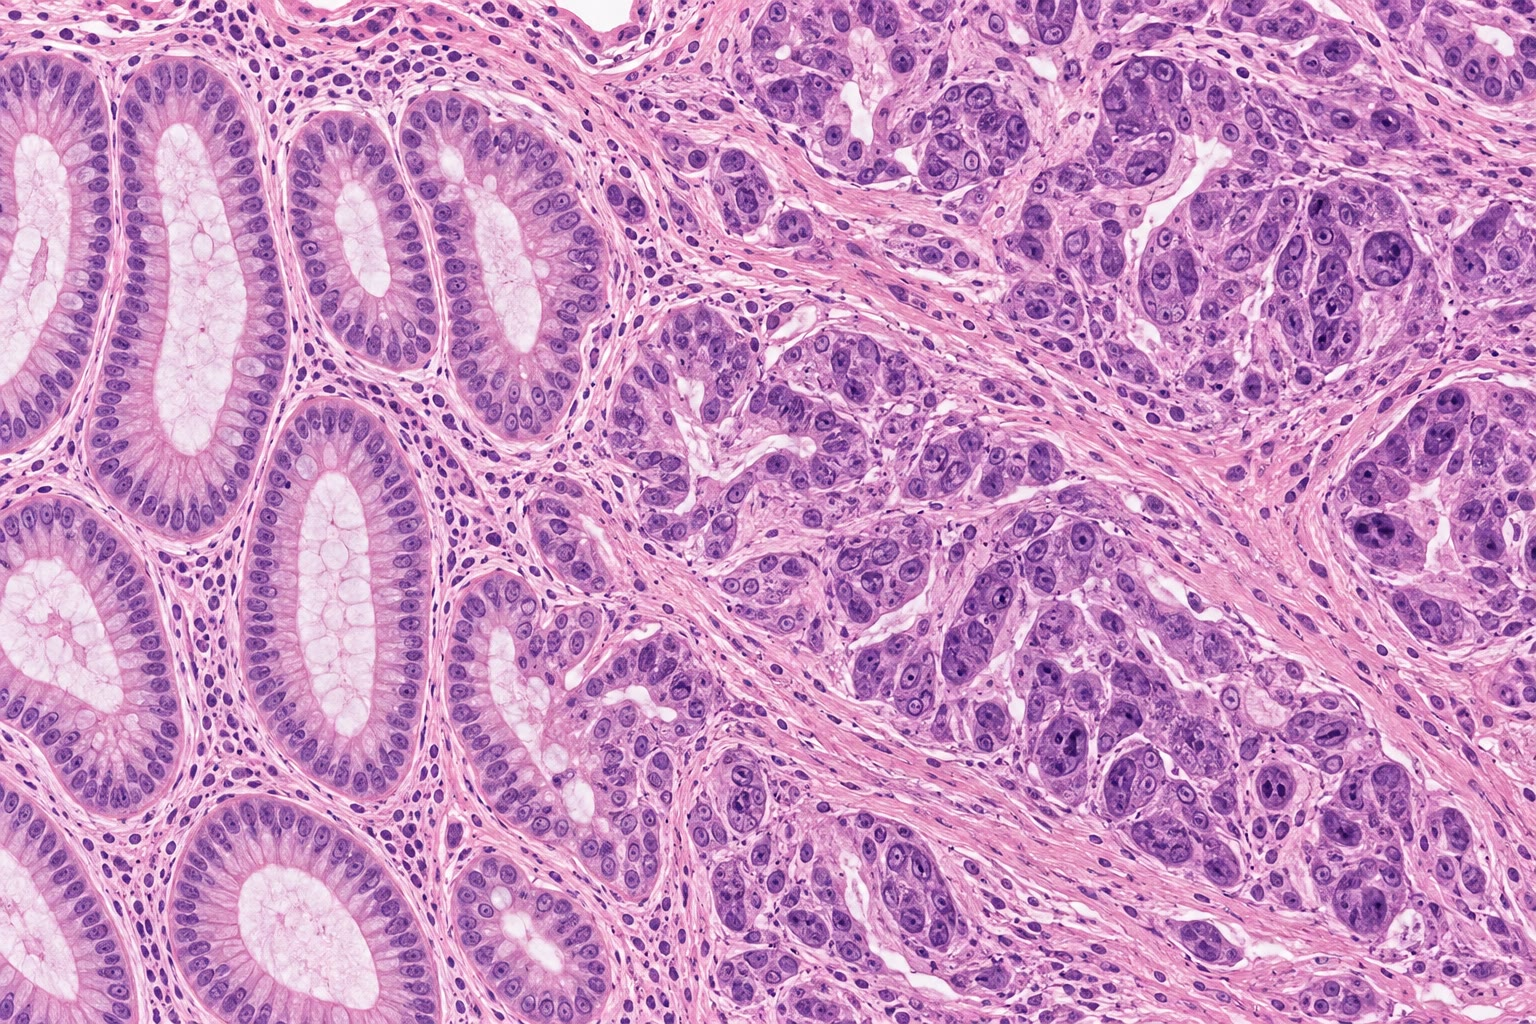
\includegraphics[width=0.56\linewidth]{images/book5/ai/b5-11-tumour-histology.jpg}

{\small A carcinoma at its border: on the left, orderly glandular
epithelium with regular nuclei; on the right, crowded cells with large,
irregular nuclei invading the underlying stroma --- the picture a
pathologist reads to call a \omterm{def:b3:cancer-biology:hallmarks}{tumour} \omterm{def:b3:cancer-biology:hallmarks}{malignant}.}
\end{omfigure}

\section{The genes that are hit}

\begin{definition}[Oncogenes and tumour suppressors]\label{def:b3:cancer-biology:genes}
\index{oncogene}\index{proto-oncogene}\index{tumour suppressor gene}\index{Ras}\index{p53}\index{two-hit hypothesis}
A \emph{proto-oncogene} is a normal gene that promotes proliferation or
survival --- a growth factor, its receptor, a signalling protein, a
transcription factor, a \omterm{def:b3:cell-cycle-apoptosis:cdk}{cyclin} --- and an \emph{oncogene} is a mutant
form that is active without its normal signal: a point mutation that
locks the \omterm{def:b3:membrane-traffic:coats}{small GTPase} \emph{Ras} in its GTP state (glycine~12 in a
quarter of all \omterm{def:b3:cancer-biology:hallmarks}{cancers}), an amplification of the gene for the receptor
HER2 or for the transcription factor Myc, a translocation that fuses
\emph{BCR} to the kinase \emph{ABL} in chronic myeloid leukaemia or puts
\emph{MYC} next to an antibody enhancer in Burkitt lymphoma. One
mutant allele suffices: oncogenes act dominantly. A \emph{\omterm{def:b3:cancer-biology:hallmarks}{tumour}
suppressor gene} restrains proliferation or enforces death or repair
--- Rb and p16 at the \omterm{def:b3:cell-cycle-apoptosis:checkpoints}{restriction point}, \emph{p53}, the guardian that
arrests or kills a damaged cell, APC in the \omterm{prop:b3:cancer-biology:pathways}{Wnt pathway} of the colon,
PTEN, BRCA1 and BRCA2, the mismatch-repair genes --- and it must lose
both alleles to contribute: \emph{two hits}, the first often inherited
in the familial \omterm{def:b3:cancer-biology:hallmarks}{cancer} syndromes, the second somatic. \emph{p53} is
mutated in half of all human \omterm{def:b3:cancer-biology:hallmarks}{cancers} and its pathway disabled in most
of the rest.
\end{definition}

\begin{proof}[Evidence]
Rous (1911) transmitted a chicken sarcoma with a cell-free filtrate,
a virus, whose single transforming gene, \emph{src}, was shown by
Varmus and Bishop (1976) to be a captured copy of a normal chicken gene
--- \omterm{def:b3:cancer-biology:genes}{oncogenes} are altered cellular genes. Weinberg (1982) transferred
DNA from a human bladder carcinoma into cultured mouse cells, which
became transformed; the responsible fragment was \emph{RAS} with a
single base change, and the same change was absent from the patient's
normal tissue. Knudson (1971) compared children with the eye \omterm{def:b3:cancer-biology:hallmarks}{tumour}
retinoblastoma: those with a family history developed several \omterm{def:b3:cancer-biology:hallmarks}{tumours}
in both eyes, early; those without developed one, later --- consistent
with the familial cases needing one somatic event, the sporadic two,
and thus with a gene whose two copies must both be lost. \emph{RB} was
cloned in 1986 and both alleles were indeed inactivated in every
\omterm{def:b3:cancer-biology:hallmarks}{tumour}.
\end{proof}

\begin{theorem}[Hits and the age curve]\label{thm:b3:cancer-biology:armitage-doll}
\index{Armitage--Doll model}\index{multistage carcinogenesis}
Suppose a \omterm{def:b3:cancer-biology:hallmarks}{cancer} requires $k$ independent, rate-limiting events in one
cell lineage, each occurring at a constant rate $u$ per cell per year,
in a population of $N$ susceptible cells, with $ut \ll 1$. Then the
probability that a given cell has suffered all $k$ events by age $t$ is
about $(ut)^{k}$, the cumulative risk in the tissue is about $N(ut)^{k}$,
and the incidence --- new cases per year at age $t$ --- is
\[
I(t) \approx N\,k\,u^{k}\,t^{\,k-1},
\]
a power of age with exponent $k - 1$: a straight line of slope $k - 1$
on a log--log plot. For an individual who inherits one of the events,
the same \omterm{def:b3:cancer-biology:hallmarks}{cancer} has incidence $\propto t^{\,k-2}$, one power lower.
\end{theorem}
\begin{proof}
Each event, at rate $u$, has occurred by time $t$ with probability
$1 - e^{-ut} \approx ut$; the events are independent, so all $k$ have
occurred with probability $(ut)^{k}$, and the order in which they
occurred does not matter here. With $N$ cells and rare events, the
expected number of cells that have completed the sequence is
$N(ut)^{k}$, and the incidence is its time derivative, $Nku^{k}t^{k-1}$.
Inheriting one event leaves $k - 1$ to occur: $(ut)^{k-1}$, incidence
$\propto t^{k-2}$. If the order of events mattered (only $1$ of $k!$
orders led to \omterm{def:b3:cancer-biology:hallmarks}{cancer}) the prefactor would change, not the exponent.
\end{proof}

\begin{example}[Reading the exponent]\label{ex:b3:cancer-biology:exponent}
The incidence of most carcinomas in adults rises as about the fifth to
sixth power of age --- from about $1$ in \num{100000} per year at
thirty to $1$ in $300$ at eighty, a factor of $300$ for a factor $2.7$
in age, and $2.7^{5.7} \approx 300$ --- which suggests six or seven
rate-limiting events. The estimate is crude: the expansion of a clone
after each hit raises the number of cells at risk of the next, so fewer
events with clonal growth between them give the same slope, and the
number of \emph{driver} mutations found in sequenced \omterm{def:b3:cancer-biology:hallmarks}{tumours} is two to
eight. Knudson's retinoblastoma fits the theorem's second statement
exactly: the sporadic disease, needing two hits, has an incidence that
rises with age (through the few years the retinoblasts exist); the
hereditary disease, needing one, is present at a nearly constant rate
from birth and strikes early and repeatedly.
\end{example}

\begin{omfigure}
\begin{tikzpicture}
\begin{axis}[
  width=0.68\linewidth, height=6cm,
  xmode=log, ymode=log,
  xmin=20, xmax=100, ymin=1e-6, ymax=1e-1,
  xlabel={age (years)}, ylabel={incidence per person per year},
  xlabel style={font=\small, at={(axis description cs:0.5,-0.12)}, anchor=north},
  ylabel style={font=\small},
  tick label style={font=\small}, xtick={20,30,50,80}, xticklabels={20,30,50,80},
  clip=false,
]
\addplot[very thick, omThm, domain=20:100, samples=2] {1e-5*(x/30)^5.7};
\addplot[very thick, omDef, domain=20:100, samples=2] {3e-4*(x/30)^1};
\addplot[very thick, omMeth!70!black, domain=20:100, samples=2] {2e-3};
\node[font=\scriptsize, omThm, anchor=south west] at (axis cs:38,2.5e-6) {carcinomas: slope $5$--$6$, six or seven events};
\node[font=\scriptsize, omDef, anchor=south west] at (axis cs:22,6e-4) {two hits: slope 1};
\node[font=\scriptsize, omMeth!70!black, anchor=south west] at (axis cs:22,2.3e-3) {one hit inherited: slope 0};
\end{axis}
\end{tikzpicture}

{\small Incidence against age on logarithmic axes. A \omterm{def:b3:cancer-biology:hallmarks}{cancer} needing $k$
rate-limiting events rises as $t^{k-1}$: the steep line of adult
carcinomas, and the two Knudson cases --- a two-hit \omterm{def:b3:cancer-biology:hallmarks}{tumour} rising
linearly, and the same \omterm{def:b3:cancer-biology:hallmarks}{tumour} in a carrier of one inherited hit, at a
constant rate from birth.}
\end{omfigure}

\begin{proposition}[The pathways that are hit]\label{prop:b3:cancer-biology:pathways}
\index{Ras--MAPK pathway}\index{PI3K pathway}\index{Wnt pathway}
The hundreds of \omterm{def:b3:cancer-biology:hallmarks}{cancer} genes fall into a dozen pathways, each of which
a \omterm{def:b3:cancer-biology:hallmarks}{tumour} disables at some point. The growth-factor pathways: a receptor
tyrosine kinase (EGFR, HER2), \omterm{def:b3:cancer-biology:genes}{Ras}, the kinase cascade Raf--MEK--ERK to
the nucleus, and in parallel PI3K--Akt--mTOR toward survival and growth,
restrained by PTEN; a \omterm{def:b3:cancer-biology:hallmarks}{tumour} activates one of them, by whichever gene.
The cell-cycle brake: \omterm{def:b3:cell-cycle-apoptosis:cdk}{cyclin} D, Cdk4, p16, Rb (\cref{ch:b3:cell-cycle-apoptosis}).
The guardian: \omterm{def:b3:cancer-biology:genes}{p53} and its regulators. Death: Bcl-2. Developmental
signalling: Wnt (APC, $\beta$-catenin) in the colon, Hedgehog in skin
and brain, Notch in T~cells. Genome maintenance: \omterm{prop:b3:dna-repair:fidelity}{mismatch repair},
\omterm{def:b3:dna-repair:dsb}{BRCA}, \omterm{def:b3:dna-repair:ddr}{ATM}. \omterm{def:b3:chromatin-epigenetics:nucleosome}{Chromatin}: the writers and remodellers of
\cref{ch:b3:chromatin-epigenetics}, mutated in a third of \omterm{def:b3:cancer-biology:hallmarks}{tumours}.
Immortality: the \omterm{def:b3:cancer-biology:telomerase}{telomerase} promoter. Because a pathway is a series of
steps, mutations in different genes are alternatives --- a \omterm{def:b3:cancer-biology:hallmarks}{tumour} with
mutant \omterm{def:b3:cancer-biology:genes}{Ras} rarely also has mutant EGFR --- and drugs against one step
can be defeated by a mutation downstream.
\end{proposition}

\begin{omfigure}
\begin{tikzpicture}[every node/.style={font=\scriptsize}, >=stealth]
  % membrane
  \draw[very thick, omDef] (0,3.6) -- (12,3.6); \draw[very thick, omDef] (0,3.3) -- (12,3.3);
  \node[above] at (1.0,3.65) {outside}; \node[below] at (1.0,3.25) {cytosol};
  % receptor
  \draw[thick, fill=omProp!35] (3.7,3.0) rectangle (4.1,4.1); \draw[thick, fill=omProp!35] (4.3,3.0) rectangle (4.7,4.1);
  \node[above, align=center] at (4.2,4.15) {growth factor $\to$ receptor kinase\\(EGFR, HER2)}; \node[right, omThm, font=\tiny] at (4.75,4.0) {amplified};
  % Ras
  \node[draw, thick, rounded corners, fill=omDef!20] (ras) at (4.2,2.3) {Ras--GTP};
  \node[right, omThm, font=\tiny] at (5.0,2.3) {G12: always on};
  \node[draw, thick, rounded corners, fill=omDef!20] (raf) at (4.2,1.4) {Raf $\to$ MEK $\to$ ERK};
  \node[right, omThm, font=\tiny] at (5.8,1.4) {BRAF V600E};
  \node[draw, thick, rounded corners, fill=omMeth!25] (myc) at (4.2,0.4) {Myc, cyclin D: proliferation};
  \node[right, omThm, font=\tiny] at (6.4,0.4) {Myc amplified};
  \draw[->, thick] (4.2,3.0) -- (ras); \draw[->, thick] (ras) -- (raf); \draw[->, thick] (raf) -- (myc);
  % PI3K branch
  \node[draw, thick, rounded corners, fill=omDef!20] (pi3k) at (9.6,2.3) {PI3K $\to$ Akt $\to$ mTOR};
  \node[draw, thick, rounded corners, fill=omMeth!25] (surv) at (9.6,0.4) {survival, growth};
  \draw[->, thick] (4.7,3.0) .. controls (6.5,2.8) .. (pi3k.north west); \draw[->, thick] (pi3k) -- (surv);
  \node[draw, thick, rounded corners, fill=omThm!15] (pten) at (12.2,1.4) {PTEN}; \draw[-|, thick, omThm] (pten) -- (9.6,1.4);
  \node[below, omThm, font=\tiny] at (12.2,1.15) {deleted};
  % p53 and Rb on the side
  \node[draw, thick, rounded corners, fill=omThm!15] (rb) at (1.2,0.4) {Rb, p16}; \draw[-|, thick, omThm] (rb) -- (myc);
  \node[below, omThm, font=\tiny, align=center] at (1.2,0.15) {both alleles lost};
  \node[draw, thick, rounded corners, fill=omThm!15] (p53) at (1.2,1.6) {p53}; \node[below, omThm, font=\tiny, align=center] at (1.2,1.35) {mutated in half\\of cancers};
  \draw[-|, thick, omThm] (p53) -- (1.2,0.65);
\end{tikzpicture}

{\small The growth-factor pathways and where \omterm{def:b3:cancer-biology:hallmarks}{cancers} hit them. Green
boxes are the outputs, blue the signalling steps that oncogenic
mutations lock on, red the suppressors that \omterm{def:b3:cancer-biology:hallmarks}{tumours} lose (bars mark
inhibition). A \omterm{def:b3:cancer-biology:hallmarks}{tumour} typically carries one activating and one or two
inactivating lesions in this diagram.}
\end{omfigure}

\section{A tumour evolves}

\begin{proposition}[Multistep carcinogenesis]\label{prop:b3:cancer-biology:multistep}
\index{driver mutation}\index{passenger mutation}\index{clonal evolution}\index{mutational signature}
A \omterm{def:b3:cancer-biology:hallmarks}{tumour} is the product of somatic evolution: mutation generates
variants, and selection within the tissue favours the ones that divide
more, die less or escape a constraint. The colorectal sequence
worked out by Vogelstein is the paradigm: loss of \emph{APC} produces
a small benign polyp; a \emph{KRAS} mutation lets it grow into an
adenoma; loss of \emph{SMAD4} or \emph{TP53} converts it to a carcinoma;
further changes allow \omterm{def:b3:cancer-biology:metastasis}{invasion}. Each step is a clonal expansion that
multiplies the cells at risk of the next. A sequenced \omterm{def:b3:cancer-biology:hallmarks}{tumour} carries
thousands of mutations, of which a handful --- typically two to eight
--- are \emph{drivers} that conferred selective advantage; the rest are
\emph{passengers}, carried along in the clone, and their spectrum is a
record of what caused them: C$\to$T at adjacent pyrimidines from
ultraviolet light in melanoma, G$\to$T from tobacco smoke in lung
\omterm{def:b3:cancer-biology:hallmarks}{cancer}, the fingerprints of the APOBEC enzymes, of defective \omterm{prop:b3:dna-repair:fidelity}{mismatch
repair}, of aflatoxin --- \emph{\omterm{prop:b3:cancer-biology:multistep}{mutational signatures}}. \omterm{def:b3:cancer-biology:hallmarks}{Tumours} are
heterogeneous, a branching tree of subclones, and the subclone that
kills is often a minority at diagnosis.
\end{proposition}

\begin{omfigure}
\begin{tikzpicture}[every node/.style={font=\scriptsize}, >=stealth]
  \foreach \x/\lab/\gene/\col/\r in {0/normal epithelium/{}/omDef!20/0.5, 2.6/small polyp/{APC lost (both alleles)}/omDef!35/0.7, 5.4/adenoma/{KRAS activated}/omProp!40/1.0, 8.4/carcinoma/{SMAD4 or TP53 lost}/omThm!35/1.3, 11.6/{invasive, metastatic}/{further drivers,\\instability}/omThm!60/1.5} {
    \draw[thick, fill=\col] (\x,0) circle (\r);
    \node[below, align=center] at (\x,-1.6) {\lab};
    \node[above, align=center, omThm] at (\x,1.6) {\gene};
  }
  \foreach \a/\b in {0.5/1.9, 3.3/4.4, 6.4/7.1, 9.7/10.1} \draw[->, very thick] (\a,0) -- (\b,0);
  \node[below] at (5.8,-2.3) {ten to thirty years; each step a clonal expansion that multiplies the cells at risk of the next};
\end{tikzpicture}

{\small The colorectal sequence. Each \omterm{prop:b3:cancer-biology:multistep}{driver mutation} expands a clone,
and the expanded clone supplies the cells in which the next driver can
arise; the whole path takes decades, which is why screening for polyps
prevents the \omterm{def:b3:cancer-biology:hallmarks}{cancer}.}
\end{omfigure}

\begin{method}[The Ames test]\label{met:b3:cancer-biology:ames}
\index{Ames test}\index{mutagen}
To test whether a chemical is mutagenic, and hence a probable
carcinogen: (1) take a strain of \emph{Salmonella} with a point mutation
in a histidine biosynthesis gene, which cannot grow without histidine;
(2) mix the chemical with a liver extract, whose enzymes convert many
compounds into their active mutagenic forms, as the body would; (3)
plate some $10^{8}$ bacteria on histidine-free agar with the mixture;
(4) count the colonies that grow --- each is a revertant in which a new
mutation restored the gene; (5) compare with the spontaneous rate. A
dose-dependent increase in revertants means the compound causes point
mutations. Most known carcinogens are positive; the test is cheap,
takes two days, and a compound that fails it is examined further
before it is made.
\end{method}

\begin{definition}[Immortality and instability]\label{def:b3:cancer-biology:telomerase}
\index{telomerase}\index{chromosomal instability}\index{aneuploidy!in cancer}
Normal somatic cells lack telomerase and count their divisions in
telomere length (\cref{ch:b3:stem-cells}): after some fifty they
senesce, and a cell that bypasses \omterm{def:b3:cell-cycle-apoptosis:other}{senescence} by losing \omterm{def:b3:cancer-biology:genes}{p53} and Rb goes
on until its telomeres are exhausted and its chromosomes fuse and break
--- a crisis that kills most clones. The rare survivor has reactivated
\emph{telomerase}, usually by a promoter mutation, and is immortal;
\qty{90}{\%} of \omterm{def:b3:cancer-biology:hallmarks}{cancers} express the enzyme. The crisis leaves scars:
fused and broken chromosomes, amplifications, deletions, translocations
--- \emph{chromosomal instability}, which, with the loss of the spindle
checkpoint and of \omterm{def:b3:cancer-biology:genes}{p53}'s response to missegregation, makes most solid
\omterm{def:b3:cancer-biology:hallmarks}{tumours} aneuploid and keeps them generating variants. A minority of
\omterm{def:b3:cancer-biology:hallmarks}{tumours} instead have a mutator phenotype from lost \omterm{prop:b3:dna-repair:fidelity}{mismatch repair},
with a normal karyotype and a thousandfold point-mutation rate.
\end{definition}

\section{The tumour as a tissue}

\begin{proposition}[Oxygen sets the size of a vessel-free tumour]\label{prop:b3:cancer-biology:oxygen}
\index{angiogenesis}\index{diffusion limit}\index{hypoxia}
Consider tissue consuming oxygen at a constant rate $q$ per unit volume,
supplied by diffusion (coefficient $D$) from a vessel at whose wall the
concentration is $c_{0}$. In one dimension at steady state, $D\,
\mathrm{d}^{2}c/\mathrm{d}x^{2} = q$, so $c(x) = c_{0} - qx^{2}/2D$ and
oxygen runs out at the distance
\[
L = \sqrt{\frac{2Dc_{0}}{q}} .
\]
With $D = \qty{2e-9}{m^2/s}$, $c_{0} = \qty{0.05}{mol/m^3}$ and $q =
\qty{0.03}{mol/m^3/s}$ (a respiring \omterm{def:b3:cancer-biology:hallmarks}{tumour}), $L \approx \qty{80}{\micro
m}$: no cell can live more than about a hundred micrometres from a
capillary. A clone with no vessels of its own therefore stops at a
diameter of one to two millimetres, its centre necrotic and its rim
alive. To grow further it must induce \emph{angiogenesis} --- its
hypoxic cells stabilise the transcription factor HIF, which induces
VEGF, which makes nearby endothelial cells sprout toward it. Judah
Folkman proposed in 1971 that blocking this step would starve \omterm{def:b3:cancer-biology:hallmarks}{tumours};
antibodies against VEGF are now standard in several \omterm{def:b3:cancer-biology:hallmarks}{cancers}, though the
\omterm{def:b3:cancer-biology:hallmarks}{tumours} adapt.
\end{proposition}
\begin{proof}
At steady state the diffusive flux $-D\,\mathrm{d}c/\mathrm{d}x$ must
change with $x$ exactly as fast as oxygen is consumed: $\mathrm{d}(-D\,
\mathrm{d}c/\mathrm{d}x)/\mathrm{d}x = -q$, that is $D c'' = q$.
Integrating twice with $c(0) = c_{0}$ and $c'(L) = 0$ at the depth
where nothing is left (no flux beyond it) gives $c = c_{0} - qx^{2}/2D$
after using $c(L) = 0$ to fix $L$. The numbers follow.
\end{proof}

\begin{omfigure}
\begin{tikzpicture}
\begin{axis}[
  width=0.6\linewidth, height=5.4cm,
  axis x line=bottom, axis y line=left,
  xmin=0, xmax=120, ymin=0, ymax=0.06,
  xlabel={distance from the capillary ($\unit{\micro m}$)}, ylabel={oxygen ($\unit{mol/m^3}$)},
  xlabel style={font=\small, at={(axis description cs:0.5,-0.12)}, anchor=north},
  ylabel style={font=\small},
  tick label style={font=\small}, xtick={0,40,80,120}, ytick={0,0.025,0.05},
  clip=false,
]
\addplot[very thick, omDef, domain=0:81.6, samples=40] {0.05 - 0.03*(x*1e-6)^2/(2*2e-9)};
\addplot[very thick, omDef, domain=81.6:120, samples=2] {0};
\fill[omThm!25] (axis cs:81.6,0) rectangle (axis cs:120,0.06);
\node[font=\scriptsize, omThm!70!black, anchor=south, align=center] at (axis cs:100,0.03) {no oxygen:\\necrosis};
\node[font=\scriptsize, omDef, anchor=south west] at (axis cs:5,0.052) {$c(x) = c_{0} - qx^{2}/2D$};
\draw[dashed, gray] (axis cs:81.6,0) -- (axis cs:81.6,0.06); \node[font=\scriptsize, anchor=south west] at (axis cs:83,0.002) {$L$};
\end{axis}
\end{tikzpicture}

{\small Oxygen in respiring tissue falls as a parabola with distance
from the nearest capillary and is exhausted at $L = \sqrt{2Dc_{0}/q}$,
about \qty{80}{\micro m} here. A \omterm{def:b3:cancer-biology:hallmarks}{tumour} without vessels is a shell of
live cells of that thickness around a dead core.}
\end{omfigure}

\begin{omfigure}
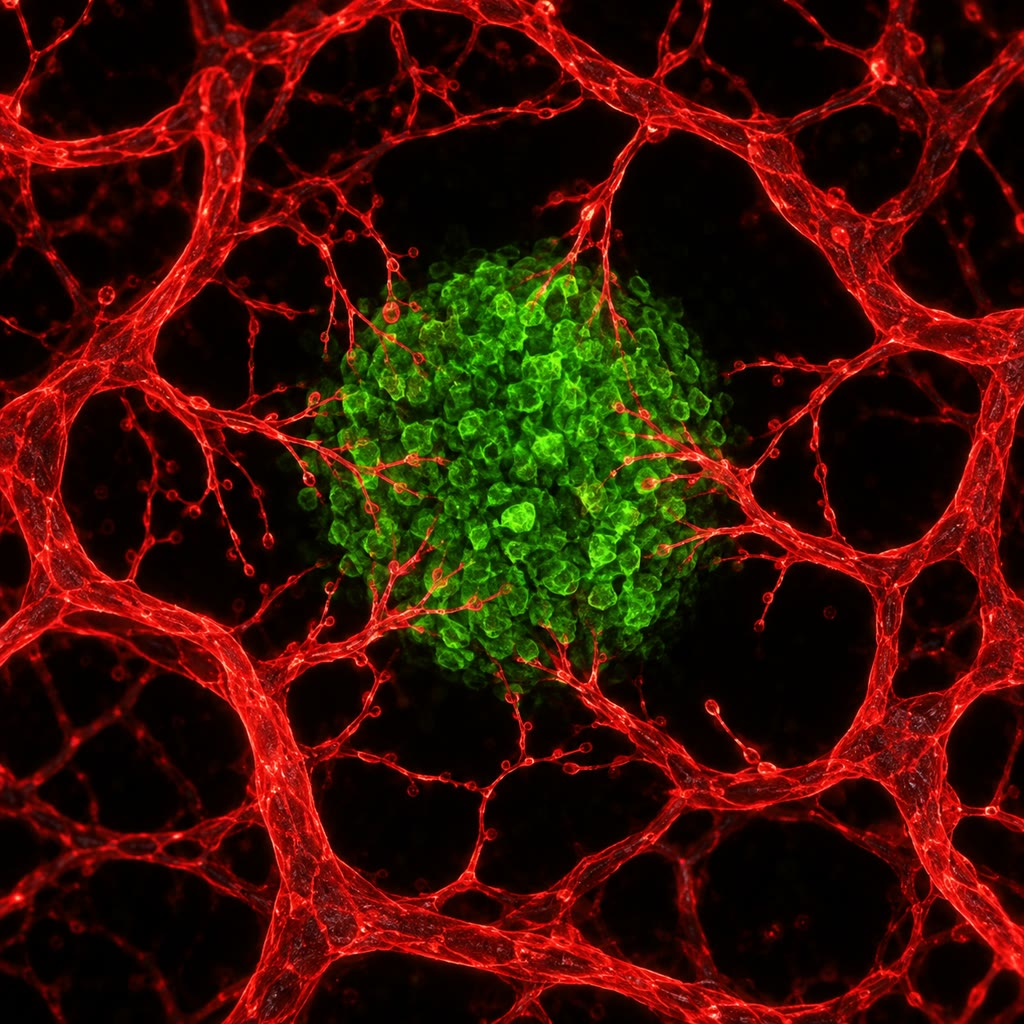
\includegraphics[width=0.36\linewidth]{images/book5/ai/b5-11-angiogenesis.jpg}\hspace{0.04\linewidth}
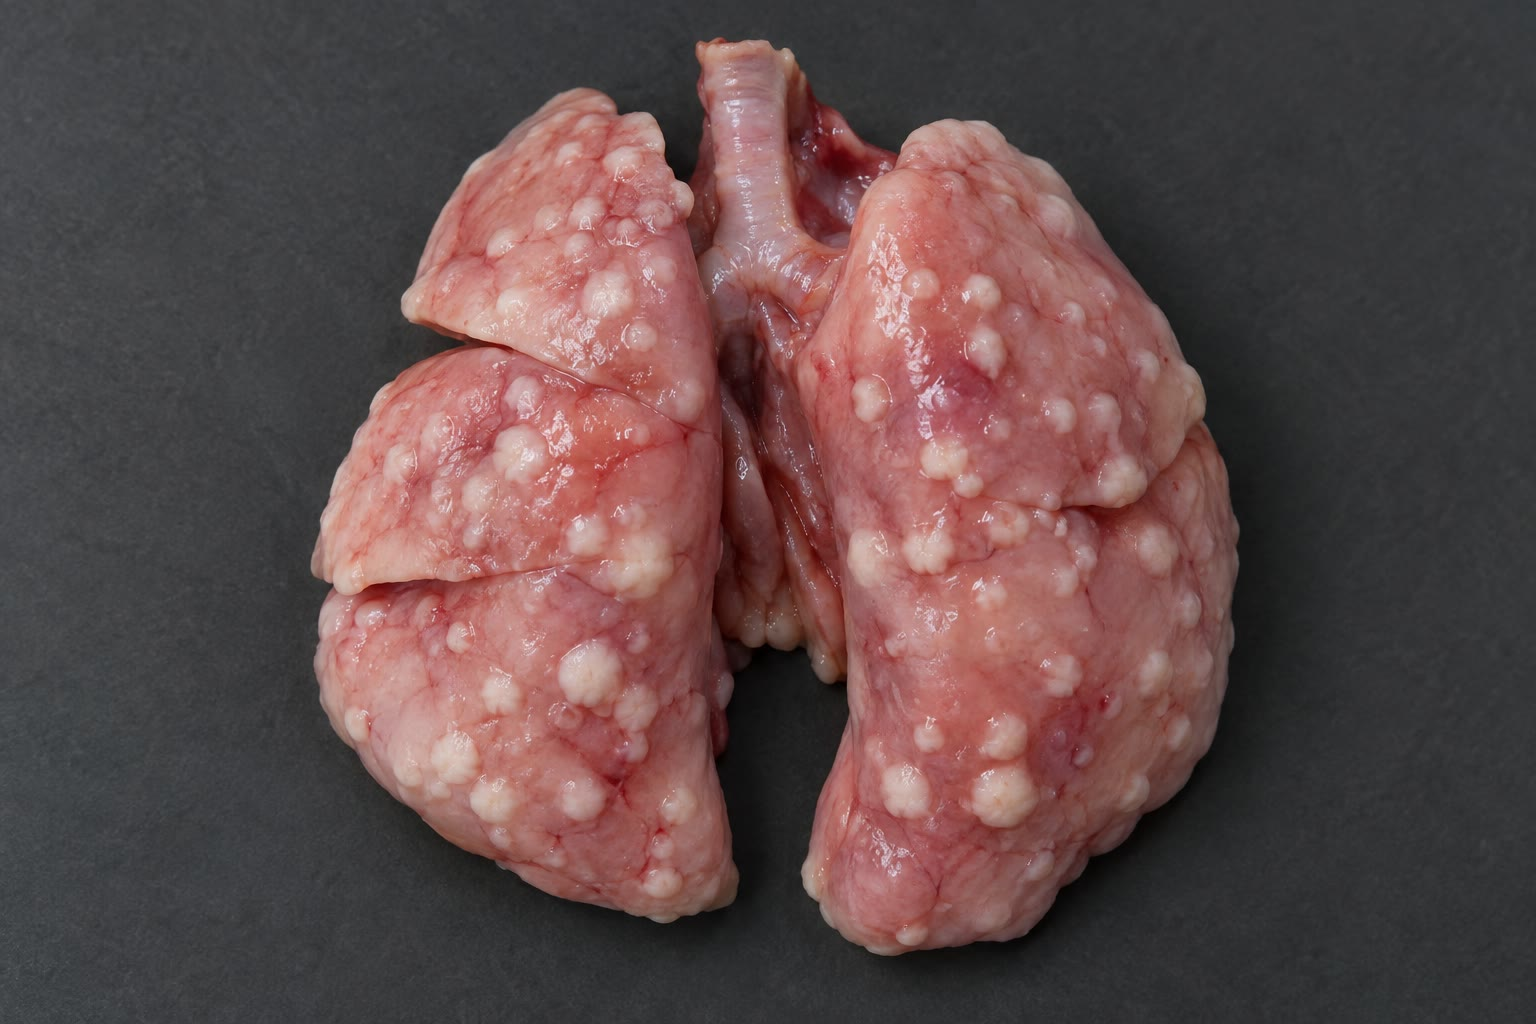
\includegraphics[width=0.54\linewidth]{images/book5/ai/b5-11-metastasis-lung.jpg}

{\small Left: a \omterm{def:b3:cancer-biology:hallmarks}{tumour} spheroid (green) recruiting new vessels (red)
from a neighbouring network --- angiogenesis in culture. Right: a mouse
lung studded with metastases, each colony founded by one cell that
survived the journey through the blood.}
\end{omfigure}

\begin{definition}[Invasion and metastasis]\label{def:b3:cancer-biology:metastasis}
\index{invasion}\index{epithelial--mesenchymal transition}\index{seed and soil}
To metastasise, a carcinoma cell must leave the epithelium --- lose its
cell junctions and polarity and acquire motility, an
\emph{epithelial--mesenchymal transition} driven by transcription
factors normally used in embryonic development --- degrade the basement
membrane and matrix with secreted proteases, cross the wall of a blood
or lymph vessel, survive in the circulation (fewer than one in ten
thousand do, killed by shear, by the absence of attachment, and by
natural killer cells), lodge in a capillary bed of another organ, cross
out, and grow there. Where it grows is not random: breast \omterm{def:b3:cancer-biology:hallmarks}{cancer} goes to
bone, lung, liver and brain, colon \omterm{def:b3:cancer-biology:hallmarks}{cancer} to the liver, prostate \omterm{def:b3:cancer-biology:hallmarks}{cancer}
to bone --- Paget's \emph{seed and soil} of 1889, explained partly by
blood flow and partly by the fit between the cell and the tissue's
signals. A disseminated cell may lie dormant for years before it grows,
which is why \omterm{def:b3:cancer-biology:hallmarks}{cancers} recur a decade after apparent cure. \omterm{def:b3:cancer-biology:hallmarks}{Metastasis}
causes nine deaths in ten from solid \omterm{def:b3:cancer-biology:hallmarks}{tumours}, and it is the step least
understood.
\end{definition}

\begin{proposition}[Escaping the immune system]\label{prop:b3:cancer-biology:immune}
\index{immune evasion}\index{checkpoint inhibitor}\index{neoantigen}
A \omterm{def:b3:cancer-biology:hallmarks}{tumour}'s mutations create \emph{neoantigens}, peptides no normal cell
presents, and cytotoxic T~cells recognise and kill \omterm{def:b3:cancer-biology:hallmarks}{tumour} cells --- the
reason immunosuppressed patients have more \omterm{def:b3:cancer-biology:hallmarks}{cancers} and the reason
\omterm{def:b3:cancer-biology:hallmarks}{tumours} with many mutations (melanoma, lung, mismatch-repair-deficient
colon) respond best to immunotherapy. A clinically evident \omterm{def:b3:cancer-biology:hallmarks}{tumour} is
one that has escaped: by losing the MHC molecules that present
peptides, by secreting suppressive factors, by recruiting regulatory
T~cells, and above all by expressing PD-L1, which engages the
inhibitory receptor PD-1 on T~cells and switches them off, the same
brake that normally ends an immune response
(\cref{ch:b3:adaptive-immunity}). Antibodies that block PD-1 or PD-L1,
or the earlier brake CTLA-4, release the T~cells; in a fraction of
patients --- a fifth to a half depending on the \omterm{def:b3:cancer-biology:hallmarks}{tumour} --- they produce
lasting remissions of \omterm{def:b3:cancer-biology:hallmarks}{cancers} that were untreatable, and their
side-effects are autoimmunity, the brake's other function.
\end{proposition}

\section{Causes and treatments}

\begin{proposition}[Causes]\label{prop:b3:cancer-biology:causes}
\index{carcinogen}\index{oncogenic virus}
\omterm{def:b3:cancer-biology:hallmarks}{Cancer} is caused by whatever raises the rate of the events in the
theorem or the number of cells at risk. \emph{Chemical carcinogens},
most of them mutagens after activation by the liver: the seventy
carcinogens of tobacco smoke, which cause a third of \omterm{def:b3:cancer-biology:hallmarks}{cancer} deaths and
raise the risk of lung \omterm{def:b3:cancer-biology:hallmarks}{cancer} fifteen- to twenty-five-fold; aflatoxin
from mouldy grain; asbestos, which is not a mutagen but a chronic
irritant. \emph{Radiation}: ultraviolet light for skin (the dimers of
\cref{ch:b3:dna-repair}), ionising radiation for leukaemia, thyroid
and breast. \emph{Infections}, a sixth of \omterm{def:b3:cancer-biology:hallmarks}{cancers} worldwide: the
papillomaviruses, whose proteins E6 and E7 destroy \omterm{def:b3:cancer-biology:genes}{p53} and inactivate
Rb and cause nearly all cervical \omterm{def:b3:cancer-biology:hallmarks}{cancers} (a vaccine now prevents them);
hepatitis B and C viruses in liver \omterm{def:b3:cancer-biology:hallmarks}{cancer}; Epstein--Barr virus in
lymphomas; \emph{Helicobacter pylori} in stomach \omterm{def:b3:cancer-biology:hallmarks}{cancer}, through decades
of inflammation. \emph{Inherited mutations} in a \omterm{def:b3:cancer-biology:hallmarks}{tumour} suppressor, the
first hit at birth, in some \qty{5}{\%} of \omterm{def:b3:cancer-biology:hallmarks}{cancers}. And chance: most
of the mutations in a \omterm{def:b3:cancer-biology:hallmarks}{tumour} arose from the ordinary errors of
replication, so tissues that divide most --- colon, skin, blood ---
have the most \omterm{def:b3:cancer-biology:hallmarks}{cancers}, and the risk rises with age whatever one does.
\end{proposition}

\begin{theorem}[Why one drug fails and two may not]\label{thm:b3:cancer-biology:goldie-coldman}
\index{Goldie--Coldman model}\index{drug resistance}\index{combination therapy}
Let a \omterm{def:b3:cancer-biology:hallmarks}{tumour} of $N$ cells have been produced by successive divisions
from one cell, and let a mutation conferring resistance to a given drug
arise at rate $\mu$ per cell division. Then the probability that the
\omterm{def:b3:cancer-biology:hallmarks}{tumour} contains \emph{no} resistant cell when treatment begins is about
\[
P_{0} \approx e^{-\mu N},
\]
so that for $\mu N \gg 1$ resistance pre-exists with near certainty.
For two drugs with independent resistance mechanisms, a cell resistant
to both arises at rate about $\mu_{1}\mu_{2}$ per division, and $P_{0}
\approx e^{-\mu_{1}\mu_{2}N}$: with $N = 10^{9}$ and $\mu = 10^{-7}$,
one drug faces $\mu N = 100$ resistant clones on average, two drugs a
probability of $10^{-5}$ that even one doubly resistant cell exists.
\end{theorem}
\begin{proof}[Partial proof]
Growing from $1$ to $N$ cells takes about $N$ divisions in all (a tree
with $N$ leaves has $N - 1$ internal nodes). If a resistant cell is
produced at each division with probability $\mu$ and, to a first
approximation, its descendants neither die nor outgrow the rest, the
number of resistance events is Poisson with mean $\mu N$, and the
probability of none is $e^{-\mu N}$. Independent mechanisms multiply
the per-division probabilities. The approximation neglects that early
mutants leave larger resistant clones --- the full distribution is that
of Luria and Delbr\"uck, treated in the Year~2 volume --- but the
probability of \emph{no} mutant, which is what decides whether the
\omterm{def:b3:cancer-biology:hallmarks}{tumour} can be cured, is exactly the Poisson term.
\end{proof}

\begin{example}[Therapies and their logic]\label{ex:b3:cancer-biology:therapy}
Surgery and radiotherapy remove or kill a localised \omterm{def:b3:cancer-biology:hallmarks}{tumour}; radiation
kills by \omterm{def:b3:dna-repair:lesions}{double-strand breaks}, and its fractionation into daily doses
lets normal tissue repair between them (\cref{ch:b3:dna-repair}).
Cytotoxic chemotherapy --- alkylating agents, antimetabolites,
\omterm{def:b3:cytoskeleton-motility:filaments}{microtubule} poisons, topoisomerase inhibitors --- kills dividing cells
of any kind, \omterm{def:b3:cancer-biology:hallmarks}{tumour} cells slightly more, and follows a
\emph{log-kill} law: each course kills a constant fraction, say
\qty{99}{\%}, so that six courses reduce $10^{12}$ cells to one, and
the same six courses are needed whether the \omterm{def:b3:cancer-biology:hallmarks}{tumour} is large or small;
the patient's hair, gut and marrow, which also divide, set the dose.
Targeted therapy attacks a lesion the \omterm{def:b3:cancer-biology:hallmarks}{tumour} depends on: imatinib
blocks the BCR--ABL kinase and turned chronic myeloid leukaemia from a
fatal disease into a chronic one; trastuzumab binds HER2; the PARP
inhibitors, the Cdk4/6 inhibitors and venetoclax of earlier chapters
each exploit one defect. Immunotherapy releases the T~cells. And the
theorem says how they should be used: in combination, early, when $N$
is smallest --- which is what adjuvant chemotherapy after surgery does
--- and with drugs whose resistance mechanisms do not overlap. The
\omterm{def:b3:cancer-biology:hallmarks}{tumour} is an evolving population, and treatment is selection.
\end{example}

\begin{omfigure}
\begin{tikzpicture}
\begin{axis}[
  width=0.7\linewidth, height=5.6cm,
  axis x line=bottom, axis y line=left,
  xmin=0, xmax=8, ymin=1, ymax=1e13, ymode=log,
  xlabel={courses of chemotherapy}, ylabel={tumour cells},
  xlabel style={font=\small, at={(axis description cs:0.5,-0.12)}, anchor=north},
  ylabel style={font=\small},
  tick label style={font=\small}, xtick={0,2,4,6,8},
  clip=false,
]
\addplot[very thick, omDef, mark=*, mark size=1.2pt] coordinates {(0,1e12) (1,1e10) (2,1e8) (3,1e6) (4,1e4) (5,1e2) (6,1)};
\addplot[very thick, omThm, mark=*, mark size=1.2pt] coordinates {(0,1e12) (1,1.01e10) (2,1.02e8) (3,1.04e6) (4,1.1e4) (5,200) (6,300) (7,600) (8,1200)};
\addplot[dashed, gray, domain=0:8, samples=2] {1e9};
\node[font=\scriptsize, gray, anchor=south west] at (axis cs:0.2,1.3e9) {detectable, $10^{9}$};
\node[font=\scriptsize, omDef, anchor=south west] at (axis cs:0.3,1e4) {\qty{99}{\%} kill per course};
\node[font=\scriptsize, omThm, anchor=south west] at (axis cs:5.2,3e3) {one resistant cell at the start: relapse};
\end{axis}
\end{tikzpicture}

{\small The log-kill law. Each course kills the same fraction of cells,
so the \omterm{def:b3:cancer-biology:hallmarks}{tumour} shrinks by a fixed number of decades per course and is
undetectable long before it is gone (blue); a single pre-existing
resistant cell survives every course and regrows (red).}
\end{omfigure}

\begin{remark}[What has changed]\label{rem:b3:cancer-biology:changed}
Half of all patients diagnosed with \omterm{def:b3:cancer-biology:hallmarks}{cancer} in a rich country now
survive ten years, against a quarter in 1970. The gain came from
prevention (tobacco, hepatitis and papillomavirus vaccines, screening
for polyps and cervical lesions), from earlier detection, and from
treatments that follow from the biology of this chapter --- the
combination chemotherapy that cures most childhood leukaemias and
testicular \omterm{def:b3:cancer-biology:hallmarks}{cancers}, the targeted drugs, and the immunotherapies. What
has not changed is metastatic disease, which the biology explains but
does not yet cure; the next gains will come from treating the \omterm{def:b3:cancer-biology:hallmarks}{tumour} as
what it is, a population evolving under the selection that treatment
imposes.
\end{remark}

\section{Exercises}

\begin{exercise}[$\star$]\label{exo:b3:cancer-biology:1}
Distinguish an \omterm{def:b3:cancer-biology:genes}{oncogene} from a \omterm{def:b3:cancer-biology:genes}{tumour suppressor gene} in mechanism,
in the number of alleles that must change, and with two examples each.
\end{exercise}

\begin{exercise}[$\star$]\label{exo:b3:cancer-biology:2}
List the \omterm{def:b3:cancer-biology:hallmarks}{hallmarks of cancer} and, for each, name one gene of this or an
earlier chapter whose alteration provides it.
\end{exercise}

\begin{exercise}[$\star$]\label{exo:b3:cancer-biology:3}
What did Knudson observe about hereditary and sporadic retinoblastoma,
and what did he infer?
\end{exercise}

\begin{exercise}[$\star$]\label{exo:b3:cancer-biology:4}
Explain the \omterm{met:b3:cancer-biology:ames}{Ames test} and why a liver extract is added.
\end{exercise}

\begin{exercise}[$\star\star$]\label{exo:b3:cancer-biology:5}
The incidence of a \omterm{def:b3:cancer-biology:hallmarks}{cancer} is $2\times 10^{-5}$ per year at age $40$
and $2\times 10^{-3}$ at age $80$. Estimate the exponent of the
age-power law and the number of rate-limiting events it suggests.
\end{exercise}

\begin{exercise}[$\star\star$]\label{exo:b3:cancer-biology:6}
Using \cref{prop:b3:cancer-biology:oxygen} with $D =
\qty{2e-9}{m^2/s}$ and $c_{0} = \qty{0.05}{mol/m^3}$, compute $L$ for
tissue consuming \qty{0.01}{mol/m^3/s} and for a \omterm{def:b3:cancer-biology:hallmarks}{tumour} consuming three
times as much. Why does a fast-growing \omterm{def:b3:cancer-biology:hallmarks}{tumour} become necrotic sooner?
\end{exercise}

\begin{exercise}[$\star\star$]\label{exo:b3:cancer-biology:7}
A \omterm{def:b3:cancer-biology:hallmarks}{tumour} of $10^{11}$ cells is treated with a drug that kills
\qty{99.9}{\%} per course. How many courses to reduce it below one
cell? Why is the \omterm{def:b3:cancer-biology:hallmarks}{tumour} undetectable after two courses although
$10^{5}$ cells remain, and what does that imply for stopping treatment?
\end{exercise}

\begin{exercise}[$\star\star$]\label{exo:b3:cancer-biology:8}
Explain why a mutation in EGFR and a mutation in KRAS are rarely
found in the same lung \omterm{def:b3:cancer-biology:hallmarks}{tumour}, and why a \omterm{def:b3:cancer-biology:hallmarks}{tumour} treated with an EGFR
inhibitor often relapses with a KRAS mutation.
\end{exercise}

\begin{exercise}[$\star\star$]\label{exo:b3:cancer-biology:9}
The papillomavirus proteins E6 and E7 inactivate \omterm{def:b3:cancer-biology:genes}{p53} and Rb. Explain
how this drives cervical \omterm{def:b3:cancer-biology:hallmarks}{cancer}, why it takes decades, and why a
vaccine given before sexual activity prevents it.
\end{exercise}

\begin{exercise}[$\star\star\star$]\label{exo:b3:cancer-biology:10}
Extend the Armitage--Doll argument to allow each hit to expand its
clone by a factor $g$ before the next: show that the incidence has the
same power of $t$ but a prefactor multiplied by $g^{k-1}$, and discuss
why the fitted $k$ from an age curve is an upper bound on the number of
drivers.
\end{exercise}

\begin{exercise}[$\star\star\star$]\label{exo:b3:cancer-biology:11}
With \cref{thm:b3:cancer-biology:goldie-coldman}, compare (a) treating a
$10^{9}$-cell \omterm{def:b3:cancer-biology:hallmarks}{tumour} with drug A for six courses then drug B for six,
and (b) giving A and B together from the start, when $\mu_{A} =
\mu_{B} = 10^{-7}$. Compute $P_{0}$ for each strategy and explain why
early combination is the rule.
\end{exercise}

\begin{exercise}[$\star\star\star$]\label{exo:b3:cancer-biology:12}
Peto's paradox: an elephant has a hundred times as many cells as a
human and lives as long, yet has no more \omterm{def:b3:cancer-biology:hallmarks}{cancer}. Using the theorem of
this chapter, say what the naive expectation is, and propose two
mechanisms by which large animals could have solved the problem (the
elephant has twenty copies of \emph{TP53}).
\end{exercise}

\section{Problem: The Arithmetic of a Tumour}

\begin{problem}[{Weekend problem --- a tumour grown from one cell and
timed to detection, its age curve read for the number of hits, its
oxygen supply and necrotic core computed, and its treatment planned
against the certainty of resistance, ending on the years to detection,
the depth of living tumour around a vessel and the probability that a
combination cures}]
\label{pb:b3:cancer-biology:1}
Data: a \omterm{def:b3:cancer-biology:hallmarks}{tumour} cell has volume \qty{1000}{\micro m^3}; doubling time
\qty{100}{days}; detection at \qty{1}{cm^3}; lethal burden \qty{1}{kg}.
Age curve: incidence $1\times 10^{-5}$ per year at $30$ and $3\times
10^{-3}$ at $80$. Oxygen: $D = \qty{2e-9}{m^2/s}$, $c_{0} =
\qty{0.05}{mol/m^3}$, $q = \qty{0.03}{mol/m^3/s}$ in \omterm{def:b3:cancer-biology:hallmarks}{tumour}; capillaries
in a vascularised \omterm{def:b3:cancer-biology:hallmarks}{tumour} are \qty{150}{\micro m} apart. Therapy: each
course kills \qty{99}{\%}; resistance mutation rate $10^{-7}$ per
division per drug; a course every three weeks; the \omterm{def:b3:cancer-biology:hallmarks}{tumour} regrows
between courses with the same doubling time.

\medskip
\noindent\textbf{Part I --- Growth.}
\begin{enumerate}
  \item How many cells in \qty{1}{cm^3}? How many doublings from one
        cell?
  \item How many years from the founding cell to detection?
  \item How many doublings, and years, from detection to the lethal
        burden? Compare the two intervals.
  \item Many \omterm{def:b3:cancer-biology:hallmarks}{tumours} are detected at \qty{1}{cm^3} but were growing for
        only five years. What must have been true of the doubling time
        early on, or of the growth law?
  \item Only a fraction $f$ of cells in a \omterm{def:b3:cancer-biology:hallmarks}{tumour} are dividing at any
        time (the growth fraction), and a fraction dies. If cells cycle
        in \qty{2}{days} but the \omterm{def:b3:cancer-biology:hallmarks}{tumour} doubles in $100$, what does
        that say about the balance of birth and death?
  \item Why does the same log-kill chemotherapy spare a slowly
        growing \omterm{def:b3:cancer-biology:hallmarks}{tumour} more than a fast one, and yet the fast one
        regrow faster between courses?
\end{enumerate}

\medskip
\noindent\textbf{Part II --- Hits.}
\begin{enumerate}[resume]
  \item From the two incidences, compute the exponent $k - 1$ of the
        age curve and the implied number of events $k$.
  \item If each event occurs at $u = 10^{-6}$ per cell per year in
        $N = 10^{8}$ susceptible cells, what does the theorem predict
        for the cumulative risk by age $70$ with your $k$? Is it
        plausible? What is missing?
  \item Repeat with clonal expansion by a factor $g = 100$ after each
        of the first $k - 1$ hits, using
        \cref{exo:b3:cancer-biology:10}.
  \item A carrier inherits one hit. By what factor is her incidence at
        age $40$ raised, if the other rates are unchanged? (Compare
        $(ut)^{k-1}$ with $(ut)^{k}$ at $t = 40$.)
  \item Smoking multiplies $u$ for one of the events by $10$. By what
        factor does the incidence rise if that event is one of $k$;
        if it is two of them?
  \item Explain why stopping smoking at fifty lowers the risk of lung
        \omterm{def:b3:cancer-biology:hallmarks}{cancer} below that of a continuing smoker, but never to that of
        a never-smoker.
\end{enumerate}

\medskip
\noindent\textbf{Part III --- Supply.}
\begin{enumerate}[resume]
  \item Compute the oxygen penetration depth $L$ in the \omterm{def:b3:cancer-biology:hallmarks}{tumour}.
  \item A vessel-free spheroid: what is the maximum diameter at which
        every cell is oxygenated? What is the thickness of the living
        rim of a \qty{2}{mm} spheroid, and what fraction of its volume
        is alive?
  \item In a vascularised \omterm{def:b3:cancer-biology:hallmarks}{tumour} with capillaries \qty{150}{\micro m}
        apart, is every cell oxygenated? Which cells are hypoxic, and
        why does that matter for radiotherapy (oxygen fixes radiation
        damage) and for selection of p53-mutant cells?
  \item A drug halves the \omterm{def:b3:cancer-biology:hallmarks}{tumour}'s capillary density. Recompute the
        spacing and say what happens to the cells midway between
        vessels.
  \item Hypoxic cells switch to glycolysis, making \qty{2}{ATP} per
        glucose instead of $30$. By what factor must they raise glucose
        uptake to keep their ATP supply, and how is this exploited in
        imaging \omterm{def:b3:cancer-biology:hallmarks}{tumours}?
  \item Explain why anti-angiogenic therapy alone rarely cures but can
        help chemotherapy reach the \omterm{def:b3:cancer-biology:hallmarks}{tumour}.
\end{enumerate}

\medskip
\noindent\textbf{Part IV --- Treatment.}
\begin{enumerate}[resume]
  \item A \qty{1}{cm^3} \omterm{def:b3:cancer-biology:hallmarks}{tumour} is treated with one drug. How many
        courses reduce it below one cell, ignoring regrowth and
        resistance?
  \item Between courses (three weeks) the survivors regrow. By what
        factor? Recompute the net kill per cycle and the number of
        cycles needed.
  \item Compute the expected number of cells resistant to the drug at
        the start of treatment and the probability that there is none.
  \item Two drugs with independent mechanisms are given together.
        Probability that no doubly resistant cell exists at the start?
        At a \omterm{def:b3:cancer-biology:hallmarks}{tumour} of $10^{12}$ cells?
  \item Adjuvant therapy is given after surgery, when perhaps $10^{6}$
        cells remain undetected. Recompute the probabilities for one
        and two drugs, and state the lesson.
  \item An immunotherapy induces T~cells that kill any cell presenting
        a neoantigen. Why is resistance to it a different problem from
        resistance to a kinase inhibitor, and which \omterm{def:b3:cancer-biology:hallmarks}{tumours} does the
        theorem suggest it should work best on?
  \item Summarise: the years from founding cell to detection
        (question~2), the depth of living \omterm{def:b3:cancer-biology:hallmarks}{tumour} around a vessel
        (question~13), and the probability that the two-drug
        combination faces no resistant cell in a \qty{1}{cm^3} \omterm{def:b3:cancer-biology:hallmarks}{tumour}
        (question~22).
\end{enumerate}
\end{problem}
